
The \textit{Compute} stage implements the calculation of the security metric and takes the measurement of the current state. 

The surveys covered in Section \ref{sec:litreview} describe properties common to all the security metrics they consider, which become evaluation criteria for their review. All security metrics inherit from a parent metric class that defines these common properties and the current system model, along with housekeeping functions and metadata like citations and usage.The security metric does not contain logic to create the inputs it operates on, so we can stack metrics to run in parallel against a single source of facts, or chain them in a processing pipeline to compose more complex analytics. 

% Our architecture for implementing security metrics is straight forward. We declare a \textit{base security metric} type from which all metrics inherit three methods: 
% \begin{itemize}
% \item Check Prerequisites: is invoked either directly by the caller or in the calculate method to ensure all items necessary for the calculation are present.
% \item Calculate: returns the resulting measurement
% \item Get Metadata: returns the environment and ancillary data used during the calculation. 
% \end{itemize}
 

% \begin{figure}[H]
% \centering
% 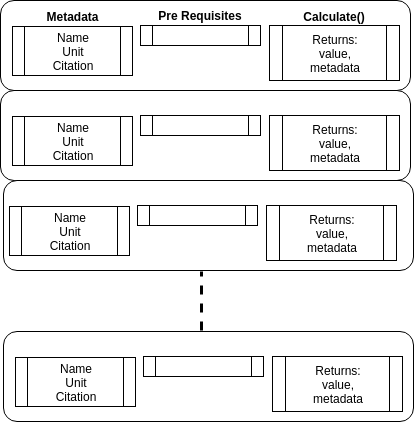
\includegraphics[width=.7\linewidth]{img/SecMet_archs.png}
% \caption{Security Metric Catalog (\textbf{SecMet})}
% \label{fig:automation:metric_arch}
% \end{figure} 

% As shown in Figure \ref{fig:automation:metric_arch}, this design allows us to implement a library of security metrics with a standard, stateless interface.


% The attack graphs described in the literature vary somewhat in structure among implementations. For example, the AGs presented in \cite{Ou_Appel_2005} include non-exploits along with exploits as nodes with edges representing lateral movements. In \cite{Noel_Jajodia_2014} the non-exploit nodes don't appear to be present in the publication, although the TVA tool isn't publicly available to test this. In \cite{Dacier_1994} and \cite{Ortalo_1999} nodes represent system privileges and edges contain exploits that grant an attacker additional privileges on a set of systems, while in \cite{Phillips_Swiler_1998} edges carry probabilities of exploitation and the nodes represent actual hosts. While the differences are subtle, they are enough to necessitate a general form of attack graph which we present in Figure \ref{fig:automation:ag_uml}. Our representation of an attack graph is a multi-edged directed acyclic graph.     

% % % \begin{wrapfigure}[10]{I}{.25\textwidth}
% % \begin{figure}[H]
% % \centering
% % 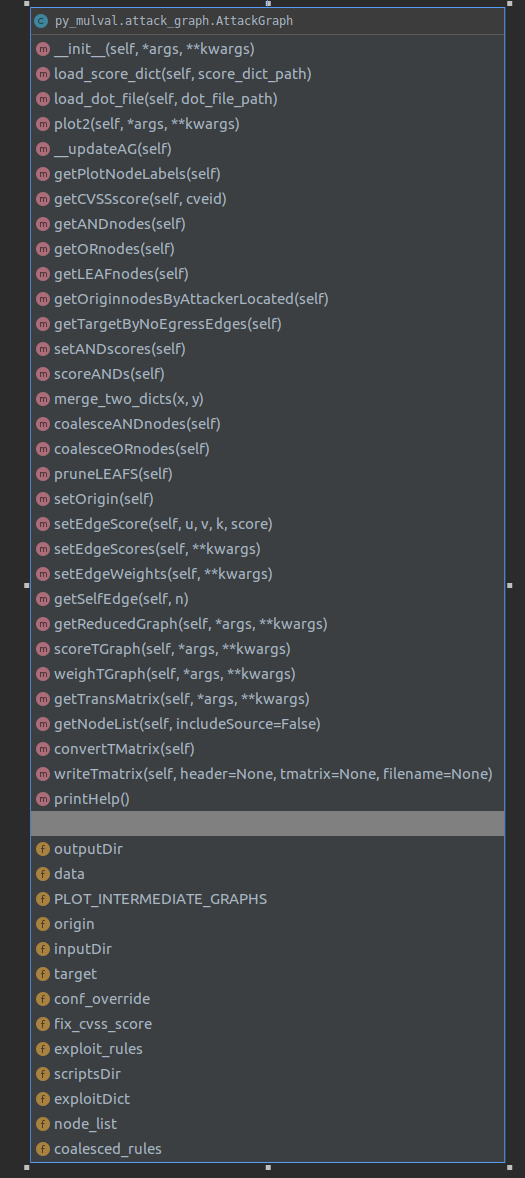
\includegraphics[scale=.45]{resource/img/ch_automation/attack_graph_class_diag.png}
% % % \end{wrapfigure}
% % \caption{Attack Graph Methods and Properties}
% % \label{fig:automation:ag_details_uml}
% % \end{figure}

% As shown in Figure \ref{fig:automation:ag_details_uml}, our implementation allows us to load various AG formats from graph description language (.dot) files, from adjacency lists as shown in Tables \ref{tab:eg_verts} and \ref{tab:eg_arcs}, or other formats as specified. Once loaded, we provide programmatic access to manipulate scoring and weighting functions, exploits definitions, and vulnerability scores. This allows for a simple means to test the range of values a metric will generate, the sensitivity of a metric to fluctuations in parameters, and how well a metric performs on different models. It also gives us some insights into how well each AG type actually models threat and defense attributes.